% EPL master thesis covers template
\PassOptionsToPackage{svgnames}{xcolor}
\documentclass{template/EPL-master-thesis-covers-EN}
\usepackage{fancyhdr}
\usepackage{tabularx}
\usepackage{geometry}
\usepackage{rotating}
\usepackage{minitoc}
\usepackage{verbatim}
\usepackage{pdfpages}
\usepackage{float}
\usepackage{caption}
\usepackage{graphics}
\usepackage{graphicx}
\usepackage{geometry}
\usepackage{mathtools}
\usepackage{amsmath}
\usepackage{amssymb}
\usepackage{newtxtext,newtxmath}
\usepackage{siunitx}
\usepackage{float}
\usepackage[inkscapeformat=pdf]{svg}
\usepackage[backend=bibtex, style=ieee]{biblatex}
\usepackage{csquotes}
\usepackage{hyperref}
\usepackage[acronym]{glossaries}
\usepackage{pgfplots}
\pgfplotsset{compat=1.18}
\usepackage{tikz}
\usetikzlibrary{positioning,fit,calc,arrows.meta,backgrounds}
\usepackage[most]{tcolorbox}
\usepackage[newfloat]{minted}
\usepackage[svgnames]{xcolor}
\usepackage{booktabs}
\usepackage{tabularx}
\usepackage{adjustbox}

% Please fill in the following boxes
% Title of the thesis
\title{Direct device access from the smartNIC towards datacenters disaggregation}

% Subtitle - remove this line if not applicable
\subtitle{Optional subtitle}

% Name of the student author(s)
\author{Nicolas \textsc{Jeanmenne}}
% \secondauthor{Firstname \textsc{Lastname}}		% remove if not applicable
%\thirdauthor{Firstname \textsc{Lastname}}			% remove if not applicable

% Official title of the master degree (copy/paste from list below)
% Master [120] in Biomedical Engineering
% Master [120] in Chemical and Materials Engineering
% Master [120] in Civil Engineering
% Master [120] in Computer Science
% Master [120] in Computer Science and Engineering
% Master [120] in Cybersecurity
% Master [120] in Data Sciences Engineering
% Master [120] in Data Science: Information technology
% Master [120] in Electrical Engineering
% Master [120] in Electro-mechanical Engineering
% Master [120] in Mathematical Engineering
% Master [120] in Mechanical Engineering
% Master [120] in Physical Engineering
% Master [60] in Computer Science
% Specialised master in nanotechnologies
% Specialised master in nuclear engineering
\degreetitle{Master [120] in Computer Science}

% Name of the supervisor(s)
\supervisor{Tom \textsc{Barbette}}
% \secondsupervisor{Firstname \textsc{Lastname}}		% remove if not applicable
%\thirdsupervisor{Firstname \textsc{Lastname}}		% remove if not applicable

% Name of the reader(s)
\readerone{Nikita \textsc{Tyunyayev}}
\readertwo{Vany \textsc{Ingezi}}			% remove if not applicable
% \readerthree{Firstname \textsc{Lastname}}			% remove if not applicable
%\readerfour{Firstname \textsc{Lastname}}			% remove if not applicable
%\readerfive{Firstname \textsc{Lastname}}			% remove if not applicable

% Academic year (update if necessary)
\years{2025--2026}

\newcommand{\authcite}[1]{\citeauthor{#1} \cite{#1}}
% Inline review comments from Nikita: \nt{text}
% Set \showcommentsfalse to hide all comments in the final version
\newif\ifshowcomments
\showcommentstrue
\definecolor{cmtcolor}{HTML}{C0392B}
\definecolor{cmtnico}{HTML}{049d1b}
\newtcbox{\cmtbadge}{on line, colback=cmtcolor, colframe=cmtcolor,
    coltext=white, fontupper=\sffamily\bfseries\scriptsize,
    arc=3pt, boxrule=0pt, boxsep=0pt, left=3pt, right=3pt, top=1.5pt, bottom=1.5pt}
\newtcbox{\cmtbadgenico}{on line, colback=cmtnico, colframe=cmtnico,
    coltext=white, fontupper=\sffamily\bfseries\scriptsize,
    arc=3pt, boxrule=0pt, boxsep=0pt, left=3pt, right=3pt, top=1.5pt, bottom=1.5pt}
\newcommand{\nt}[1]{\ifshowcomments\cmtbadge{NT}\,{\color{cmtcolor}\sffamily\small\itshape #1}\fi}
\newcommand{\nj}[1]{\ifshowcomments\cmtbadgenico{NJ}\,{\color{cmtnico}\sffamily\small\itshape #1}\fi}
\makeglossaries
\newacronym{spdk}{SPDK}{Storage Performance Development Kit}
\newacronym{aio}{AIO}{Asynchronous Input/Output}
\newacronym{bdev}{BDEV}{Block device}
\newacronym{npf}{NPF}{Network Performance Framework}
\newacronym{fio}{FIO}{Flexible I/O tester}
\newacronym{fish}{Fish}{Friendly Interactive Shell}
\newacronym{dda}{DDA}{Direct Device Access}
\newacronym{rdma}{RDMA}{Remote Direct Memory Access}
\newacronym{cpu}{CPU}{Central Processing Unit}
\newacronym{nvme}{NVMe}{Non-Volatile Memory Express}
\newacronym{nvmeof}{NVMe-oF}{NVMe over Fabric}
\newacronym{gpu}{GPU}{Graphics Processing Unit}
\newacronym{fpga}{FPGA}{Field-Programmable Gate Array}
\newacronym{dpu}{DPU}{Data Processing Unit}
\newacronym{hca}{HCA}{Host Channel Adapter}
\newacronym{pci}{PCI}{PCI Express}
\newacronym{p2pdma}{P2PDMA}{Peer-to-Peer Direct Memory Access}
\newacronym{tcp}{TCP}{Transmission Control Protocol}
\newacronym{cisc}{CISC}{Complex Instruction Set Computer}
\newacronym{arm}{ARM}{Advanced RISC Machine}
\newacronym{mtu}{MTU}{Maximum Transmission Unit}
\newacronym{rtt}{RTT}{Round-Trip Time}
\newacronym{fs}{FS}{File System}
\newacronym{ma}{MA}{Monolithic Architecture}
\newacronym{da}{DA}{Disaggregated Architecture}
\newacronym{roce}{RoCE}{RDMA over Convergent Ethernet}
\newacronym{ssd}{SSD}{Solid State Drive}
\newacronym{hdd}{HDD}{Hard Disk Drive}
\newacronym{qd}{QD}{Queue Depth}
\newacronym{io}{I/O}{Input/Output}
\newacronym{hpc}{HPC}{High-Performance Computing}
\newacronym{llc}{LLC}{Last Level Cache}
\newacronym{api}{API}{Application Programming Interface}
\newacronym{dma}{DMA}{Direct Memory Access}
\newacronym{nic}{NIC}{Network Interface Card}
\newacronym{http}{HTTP}{Hypertext Transfer Protocol}
\newacronym{tls}{TLS}{Transport Layer Security}
\newacronym{pcie}{PCIe}{PCI Express}
\newacronym{dpdk}{DPDK}{Data Plane Development Kit}
\newacronym{pslc}{pSLC}{Pseudo-Single-Level Cell}
\bibliography{biblio.bib}

\newtcolorbox{tbox}[1]{
    breakable,
    colback=gray!10,
    colframe=gray!60,
    boxrule=0.5pt,
    arc=2pt,
    left=6pt,
    right=6pt,
    top=6pt,
    bottom=6pt,
    title={#1}
}

\newtcolorbox{draftbox}{
    breakable,
    colback=Goldenrod!10,
    colframe=Goldenrod!60,
    boxrule=0.5pt,
    arc=2pt,
    left=6pt,
    right=6pt,
    top=6pt,
    bottom=6pt,
    title={\textbf{DRAFT NOTES}}
}


\hypersetup{
    pdftitle={Direct device access from the smartNIC towards datacenters disaggregation},
    pdfauthor={Nicolas Jeanmenne},
    pdfsubject={Master thesis: Direct device access and datacenter disaggregation},
    pdfkeywords={smartNIC, datacenter, disaggregation, direct memory access, DMA, RDMA, NVMe},
    pdfproducer={pdflatex},
}

\tikzset{
  panel/.style={draw=black!75,line width=.8pt,rounded corners=3pt,fill=gray!5,inner sep=8pt},
  mem/.style={draw=black!75,line width=.7pt,rounded corners=2pt,fill=white},
  cell/.style={draw=black!65,line width=.55pt,fill=white,minimum width=1.05cm,
               minimum height=.48cm,font=\scriptsize,inner sep=1pt},
  cqe/.style={cell,minimum width=1.15cm},
  boxtitle/.style={font=\small\bfseries},
  cpubox/.style={mem,minimum width=1.5cm,minimum height=.65cm,font=\small\bfseries},
  dbbox/.style={mem,minimum width=1.8cm,minimum height=.50cm,font=\scriptsize\bfseries},
  engbox/.style={mem,minimum width=2.8cm,minimum height=1.0cm,align=center,font=\small\bfseries},
  flashbox/.style={mem,minimum width=2.5cm,minimum height=.75cm,font=\small\bfseries},
  bufbox/.style={mem,minimum width=4.0cm,minimum height=.9cm,align=center,font=\small\bfseries},
  arr/.style={-{Stealth[length=2.4mm,width=1.7mm]},line width=.9pt,draw=black!85},
  bi/.style={{Stealth[length=2.4mm,width=1.7mm]}-{Stealth[length=2.4mm,width=1.7mm]},line width=.9pt,draw=black!85},
  dasharr/.style={-{Stealth[length=2.4mm,width=1.7mm]},line width=.85pt,dashed,draw=black!70},
  lab/.style={inner sep=2pt,font=\scriptsize,align=center},
}

% Document
\begin{document}
% Front cover page
\thispagestyle{empty}
\maketitle

\pagestyle{empty}

\chapter*{Abstract}
\addcontentsline{toc}{chapter}{Abstract}

    \input{src/abstract.tex}

\setcounter{tocdepth}{4}
\tableofcontents
\newpage

\printglossary[title= List of acronyms, type=\acronymtype]
\newpage
\listoflistings
\newpage

\chapter{Introduction}
\pagenumbering{arabic}
\setcounter{page}{1}
\pagestyle{plain}

    TODO 

\nt{This is very important, you should work on it ASAP}
%\section{Introduction}

% For decades, servers in datacenters were designed under a monolithic model, meaning that all hardware resources are physically
% attached to the same frame. This model is now a bottleneck for performance, network throughput and to efficiently consume resources.
% In order to solve the monolithic challenge, a new architectural design has been proposed : disaggregation.



\chapter{Background} \label{ch:background}

    This chapter provides an overview of disaggregated datacenter architectures and smartNIC-to-storage interactions.  We will first give an overview of
the main concepts and definitions used in the literature, then we will review the main
architectural challenges and solutions proposed by researchers. Finally, we will list some
unresolved challenges that we aim to solve in this thesis.

~\nt{What is a SmartNIC, how does it fit in a disagragated architecture?}

\section{Overview of concepts and definitions}

High-performance disaggregated storage rely on a tightly coupled pipeline bridging storage media, network interfaces and protocols, and specialized software stacks. To understand the challenges and solutions proposed in the literature, it is important to first define the main concepts layer by layer.

% New kind of hardware components have emerged, \acrfull{ssd} are replacing traditional \acrfull{hdd}  
% These trends have enabled researchers and companies to explore new approaches to \acrfull{hpc}. Modern \acrshort{ssd}s use the \acrfull{nvme} protocol, a low-latency, high-throughput interface designed for flash storage. \acrshort{nvme} devices can be accessed over the network using \acrfull{nvmeof}, which extends the \acrlong{nvme} command set to support network fabrics (smartNICs, \dots) \cite{noauthor_nvme_2021, noauthor_what_nodate, guz_nvme-over-fabrics_2017}. Such advancements made it possible to design new architecture designs, such as disaggregated datacenters. 

% Writing efficient storage applications involves understanding the role of \acrfull{spdk}. \acrshort{spdk} is a set of tools and libraries for building high-performance storage applications, particularly those that interact with \acrshort{nvme} devices. It provides a user-space driver that bypasses the kernel, allowing for lower latency and higher throughput compared to traditional kernel-based drivers \cite{noauthor_storage_nodate}. This development kit will be used in this thesis to implement and evaluate our proposed solutions, as detailed in the next chapters.

\subsection{Storage medium and interface}

% A traditional \acrfull{hdd} is a mechanical device that stores data on spinning magnetic disks. Its performance is bounded by mechanical seek time and rotational latency, which limits its throughput and increases access time. In contrast, a \acrfull{ssd} is an electronic device that stores data on non-volatile flash memory. \cite{mecheloni_inside_2018}

% \subsubsection{Peripheral Component Interconnect Express}

% Pas oublier de faire le lien avec PCIe 5 / 6 pour en parler avec ZeroNIC.

A traditional \acrfull{hdd} is a mechanical device that stores data on spinning magnetic disks. To read or write data, the drive must physically move a mechanical arm, the read/write head, to the correct track and wait for the disk to rotate to the correct position. These mechanical movements, called seek time and rotational latency take each a few milliseconds, which limits the throughput and increases access time. Typical throughput of a \acrshort{hdd} is around 100 MB/s and one hundred requests per second.  In contrast, a \acrfull{ssd} is a device that stores data on non-volatile flash memory and contains no moving parts : accessing data is a purely electronic operation that takes tens of microseconds. Modern \acrshort{ssd}s can achieve throughput of several GB/s and hundreds of thousands to millions of requests per second, depending on how those devices are connected to the system. \acrshort{ssd}s are therefore suitable for high-performance applications as they are a thousand to ten thousand times faster than \acrshort{hdd}s. \cite{mecheloni_inside_2018, haas_what_2023}

This speedup has a consequence that motivates this thesis : the storage medium is no longer the bottleneck in the data path nor the slowest component in the system. With several millions of requests per second, the machine must process one request every few hundred nanoseconds, and the software layers such as system calls, the kernel block layer, interrupts, \dots become the new bottleneck. Understanding the storage medium and its interface is therefore crucial to design high-performance storage applications.

\subsubsection{Flash memory behavior}

Flash memory stores data in pages of a few kilobytes, which are grouped into blocks of a few megabytes. A page can be written only once before it must be erased, and an erase operation can only be performed on a whole block, so an \acrshort{ssd} cannot overwrite data in place. This behavior is called the \textit{erase-before-write}, and an internal controller is responsible to write data to a new page and erase old pages in the background. This behavior has direct consequences that reappear in chapter \ref{ch:evaluation} : write operations are slower and more complex than read operations, and continuous write throughput can drop if the \acrfull{slc} cache is exhausted. A \acrshort{slc} cache is a small portion of the \acrshort{ssd} that is used to store data in a single-level cell mode, which is faster than \acrshort{tlc} or \acrshort{qlc} used for the rest of the device. When the \acrshort{slc} cache is full, the \acrshort{ssd} must write data directly to the slower \acrshort{tlc}/\acrshort{qlc} area, which can cause a significant drop in write throughput.


\subsubsection{PCI Express and NVMe}

An \acrshort{ssd} can be connected to a computer through several interfaces, such as \acrshort{sata}, \acrshort{sas}, or \acrshort{pcie}. \acrshort{sata} and \acrshort{sas} are legacy interfaces that were designed for \acrshort{hdd}s, and are therefore limited in terms of throughput. Modern systems connect \acrshort{ssd}s to the processor over \acrfull{pcie}, a high-speed point-to-point interconnect that allows for low-latency, high-throughput communication between devices .\acrshort{pcie} has evovled into several generations, \acrshort{pcie} 3.0 transfers rougly 1 GB/s per lane, \acrshort{pcie} 4.0 about 2 GB/s per lane, \acrshort{pcie} 5.0 about 4 GB/s per lane, and \acrshort{pcie} 6.0 about 8 GB/s per lane \cite{pcie-1-5-bit-rates,pcie-6-specs}. A typical \acrshort{ssd} or \acrfull{nic} uses four lanes (x4) so \acrshort{pcie} 4.0 provides a total throughput of about 8 GB/s. The \acrshort{pcie} generation and lanes count thus determine the hard ceiling a storage device or network interface can achieve. \acrshort{pcie} also allows for \acrfull{dma} to and from devices, which allows for direct memory access without CPU involvement, further reducing latency and improving throughput.

\begin{figure}[htbp]
	\centering
	\adjustbox{max width=0.85\columnwidth}
	{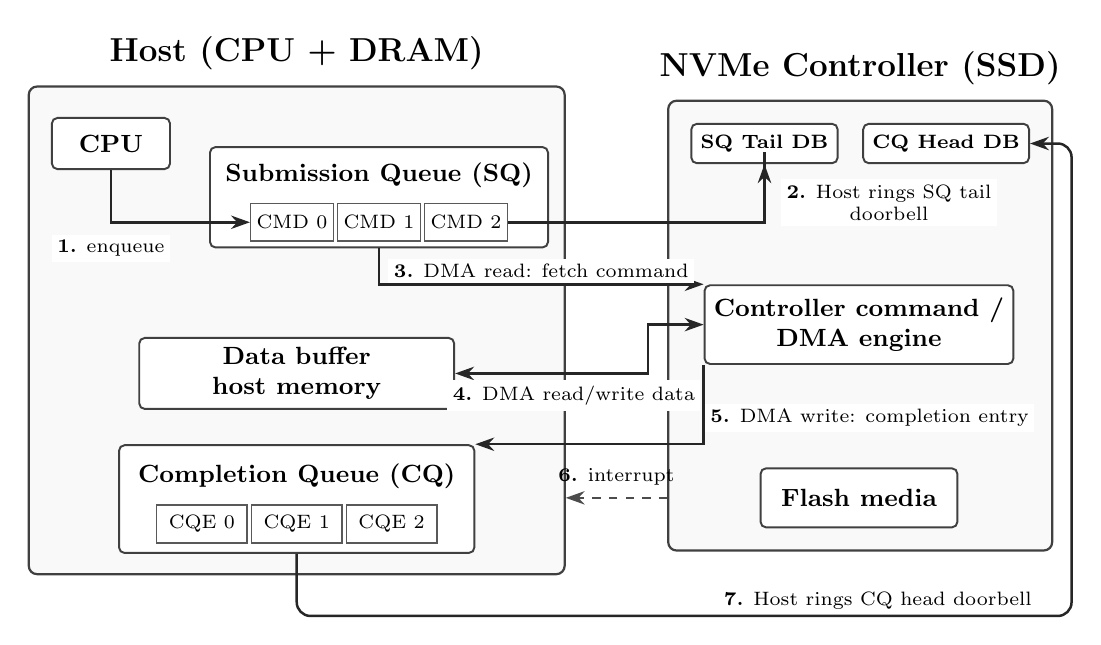
\begin{tikzpicture}
  \def\cellsep{1pt}

  \node[cpubox] (cpu) at (0.7,6.6) {CPU};

  \node[cell] (cmd0) at (3.0,5.6) {CMD 0};
  \node[cell,right=\cellsep of cmd0] (cmd1) {CMD 1};
  \node[cell,right=\cellsep of cmd1] (cmd2) {CMD 2};
  \node[boxtitle,above=2pt of cmd1] (sqtitle) {Submission Queue (SQ)};


  \node[fit=(cpu)(sqtitle)(cmd0)(cmd2),inner sep=0pt] (hostTopRef) {};

  \node[bufbox,below=12mm of hostTopRef] (buffer) {Data buffer \\host memory};

  \node[cqe,below=12mm of buffer] (cqe1) {CQE 1};
  \node[cqe,left=\cellsep of cqe1] (cqe0) {CQE 0};
  \node[cqe,right=\cellsep of cqe1] (cqe2) {CQE 2};
  \node[boxtitle,above=2pt of cqe1] (cqtitle) {Completion Queue (CQ)};

  \node[dbbox] (sqdb) at (9.0,6.6) {SQ Tail DB};
  \node[dbbox,right=3mm of sqdb] (cqdb) {CQ Head DB};
  \node[engbox] (eng) at (10.2,4.3) {Controller command /\\DMA engine};
  \node[flashbox] (flash) at (10.2,2.1) {Flash media};


  \begin{pgfonlayer}{background}
    \node[panel,inner ysep=11pt,fit=(cpu)(sqtitle)(cmd0)(cmd2)(buffer)(cqtitle)(cqe0)(cqe2)] (host) {};
    \node[mem,inner sep=2pt,fit=(sqtitle)(cmd0)(cmd2)] (sq) {};
    \node[mem,fit=(cqtitle)(cqe0)(cqe2)] (cq) {};
    \node[panel,fit=(sqdb)(cqdb)(eng)(flash)] (ctl) {};
  \end{pgfonlayer}

  \node[font=\bfseries\large,above=2pt of host] {Host (CPU + DRAM)};
  \node[font=\bfseries\large,above=2pt of ctl] {NVMe Controller (SSD)};


  \draw[arr]
    (cpu.south) |- node[pos=0.5,lab,below=4pt, fill=white] {\textbf{1.} enqueue} (cmd0.west);

  \draw[arr]
    (cmd2.east) -- (cmd2.east -| sqdb.south) |- node[pos=0.85,xshift=45pt,lab,below=5pt, fill=white] {\textbf{2.} Host rings SQ tail \\ doorbell} (sqdb.south);

  \draw[arr]
    (sq.south) |- node[pos=0.75,lab,above,fill=white] {\textbf{3.} DMA read: fetch command} (eng.north west);

  \draw[bi]
    (buffer.east) -| ([xshift=-20pt]eng.west) node[near start,lab,below=2pt,xshift=8pt,fill=white] {\textbf{4.} DMA read/write data} |- (eng.west);

  \draw[arr]
    (eng.south west) |- node[midway,lab,below,fill=white,xshift=60pt, yshift=15pt] {\textbf{5.} DMA write: completion entry} (cq.north east);

  \draw[dasharr]
    (ctl.west |- flash.west) -- node[midway,lab,above,yshift=2pt] {\textbf{6.} interrupt} (host.east |- flash.west);

  \draw[arr,rounded corners=5pt]
    (cq.south) |- (12.9,0.6)
    node[very near end,lab,above] {\textbf{7.} Host rings CQ head doorbell}
    -- (12.9,6.6) -- (cqdb.east);
\end{tikzpicture}}
	\caption{Illustration of the NVMe command submission and completion process. The host CPU enqueues commands in the \acrshort{sq}, notifies the controller via a doorbell register, and the controller fetches commands using \acrshort{dma}. Data is transferred between the host and controller using DMA, and upon completion, the controller writes a completion entry to the \acrshort{cq} and signals the host with an interrupt.}
	\label{fig:NVMe-schema}
\end{figure}



\acrfull{nvme} is a protocol designed for high-speed communication with non-volatile storage devices, such as \acrshort{ssd}s. It provides a low-latency, high-throughput interface that allows multiple commands to be processed in parallel, making it well-suited for modern storage applications. \acrshort{nvme} uses queues to manage commands and completions. Commands are submitted to the \acrshort{ssd} through \acrfull{sq}s, the \acrshort{ssd} fetches the request from main memory using \acrshort{dma}, processes the request, and places the result in a \acrfull{cq}, ready to be picked up by the host. Many queues can exist in parallel, and each queue can hold multiple commands. This queuing model is what exposes the internal parallelism of the flash chips to the host. Since a single request takes tens of microseconds, reaching millions of requests per second requires keeping hundreds of requests in flight simultaneously. The number of outstanding requests is called the \acrshort{io} depth, and it is a key parameter of our evaluation methodology in chapter \ref{ch:evaluation}. Figure \ref{fig:NVMe-schema} illustrates the \acrshort{nvme} command process.

Finally, \acrshort{nvme} was originally designed for locally attached devices over \acrshort{pcie}. The protocol has been extended to operate over \acrfull{nvmeof}, which we discuss in section \ref{sec:nvmeof}, as it is central to the SmartNIC architecture studied in this thesis.

\subsection{Network} \label{sec:nvmeof}

% High-speed network communication is a critical aspect of disaggregated architectures. \acrfull{rdma} \cite{rdma_rfc} \cite{rdma_consortium} is a protocol that allows one computer to access memory on another computer without CPU involvement, providing high throughput and low latency. \acrfull{roce} \cite{roce_nvidia_docs} is a variant of \acrshort{rdma} that operates over Ethernet networks, making it more widely compatible with existing infrastructure.


\subsection{Disaggregation}

% This thesis uses \textit{disaggregation} to denote an architecture in which hardware resources such as compute, memory,
% accelerators, and storage are split into pools (or nodes) interconnected through a high-speed network. This design allows
% resources to be allocated on demand, improving utilization and availability. Two levels are commonly distinguished.
% \textit{Partial disaggregation} separates storage from compute and memory, which remain integrated together, this level has
% already been widely implemented since the early 2020s. \textit{Full disaggregation} groups each resource type into dedicated
% clusters that communicate over the network. \cite{lin_disaggregated_2020}. Figures \ref{fig:partial-disaggregation} and \ref{fig:full-disaggregation} illustrate these two levels of disaggregation.


\begin{figure}[H]
	\centering
	\begin{minipage}{0.48\linewidth}
		\centering
		\includesvg[width=0.8\linewidth]{src/img/partial_disa.svg}
		\caption{Partial disaggregation architecture}
		\label{fig:partial-disaggregation}
	\end{minipage}
	\begin{minipage}{0.48\linewidth}
		\centering
		\includesvg[width=0.8\linewidth]{src/img/full_disa.svg}
		\caption{Full disaggregation architecture}
		\label{fig:full-disaggregation}
	\end{minipage}
\end{figure}

\subsection{Software stack}


\section{Architectural challenges}

{\color{red} I did not modify this section, you can skip it, I plan to rewrite it later.}

Architectural challenges can be grouped into two categories:

\begin{itemize}
	\item Limitations of traditional monolithic servers, which motivate the transition toward disaggregated architectures.
	\item New challenges introduced by disaggregation, which break assumptions commonly made in earlier systems research and require new design approaches.
\end{itemize}

\nt{This is too short and it lacks paper citations}

\subsection{Monolithic challenges}

The main limitation of \acrfull{ma} is \textbf{resource stranding}. When one resource is exhausted (for example, memory), other resources on the same server may remain underutilized, leading to waste.

Another important issue in \acrfull{ma} is availability under failures. A single hardware failure can impact the whole server and make it unavailable.

Finally, hardware replacement and upgrades in \acrfull{ma} often require costly maintenance operations.

\subsection{Disaggregation challenges}

In disaggregated architecture (\acrfull{da}), the network becomes the central communication path between resource clusters. This creates strict latency and bandwidth requirements: \acrshort{cpu}-storage communication typically tolerates millisecond-scale delays, whereas \acrshort{cpu}-memory communication requires nanosecond-scale delays (around 100 ns) \cite{lin_disaggregated_2020}.

Current network stacks also expose strong flexibility-performance trade-offs.~\nt{Explain a bit what is RDMA and what is RoCE} \acrshort{rdma} and \acrfull{roce} offer high performance but limited flexibility due to hardware coupling. In addition, \acrshort{rdma} can suffer from head-of-line blocking, congestion, and vendor lock-in because its requirements are not always satisfied by commodity hardware. By contrast, Linux \acrshort{tcp} is more flexible~\nt{This is too vague} but delivers lower performance and less efficient \acrshort{cpu} utilization \cite{skiadopoulos_high-throughput_2024}.


\chapter{State-of-the-art designs and solutions} \label{ch:sota}

    \section{Control and data plane separation}

% 1. Problem : monolithic TCP
%.2. Mechanism : split stack
% 3. Zero-copy data path

~\nt{Discuss how decoupling the stack helps for scalability maybe? Need to fit better in the disagragation discussion}
Standard network stacks like Linux \acrshort{tcp} force all operations to be executed on a single plane on the host \acrshort{cpu}, causing performance bottlenecks and resource contention.~\nt{sources? Claim should be backed up} To address this, researchers have proposed split stack architectures that separate control and data operations. This decoupling allows stateful control plane operations to be managed by the \acrshort{cpu}, while stateless data plane operations can be offloaded to hardware accelerators, enabling zero-copy mechanisms.~\nt{Aren't we mixing zero-copy and split stack here?} The term \textit{zero-copy} refers to data transfers between devices without requiring data replication by the CPU, thereby avoiding redundant copies and reducing CPU usage.

Recent state-of-the-art research uses this design to solve encountered bottlenecks rather than offloading every operation. A common design is to separate control operations from data operations. This is the case for \textbf{IO-TCP} \cite{kim_rearchitecting_2023}, a \acrshort{http} / \acrshort{tls} web content delivery system which splits \textit{mTCP} \cite{jeong_mtcp_2014}, a userspace stack. The control plane is responsible for connection management, congestion control, and retransmission. It runs on the host \acrshort{cpu}, while the data plane is responsible for packet preparation and transfer, running on the smartNIC. This design prevents disk \acrshort{io} pollution in the \acrshort{cpu} cache and reduces contention, notably on the \acrfull{llc} miss rate which is improved by 27 \%. This allows a single core to saturate several \acrshort{nvme} disks at 77.4 Gbps, whereas Linux and Atlas \cite{marinos_diskcryptnet_2017} (a video streaming FreeBSD server) achieve roughly half that throughput even when using 10 cores. Network performance also benefits from reduced \acrshort{rtt} and improved throughput.

\nt{This could be more high-level, too many words/concepts are not explained}

While IO-TCP addresses host-centric bottlenecks with a specialized userspace implementation, \textbf{ZeroNIC} \cite{skiadopoulos_high-throughput_2024} focuses on flexibility and generality for host networking. Rather than modifying a specific stack, ZeroNIC physically separates the control and data planes to achieve end-to-end zero-copy, and can run on host userspace, kernel, or on an accelerator. Prior approaches required strict page alignment, page remapping, or custom \acrfull{api} to avoid data copies. ZeroNIC, on the other hand, achieves zero-copy without these constraints by delegating payload placement to the \acrshort{nic} hardware. Utilizing on-NIC data structures such as memory segments and flow tables, the hardware calculates memory offsets and \acrshort{dma}s payloads directly to applications (which can reside on \acrshort{cpu}, \acrshort{dpu}, or \acrshort{fpga}). The software control plane only processes splitted headers, maintaining reliable protocol semantics, without ever touching the payload. This approach allows a single core to saturate a 100 Gbps link with a single TCP flow, while using only 17\% of a single \acrshort{cpu}.

\section{Hardware-offloaded storage}

Beyond network stack offloading, zero-copy mechanisms can also be applied to storage operations. Concerning \acrshort{nvme} storage, \textbf{Scalio} \cite{sun_scalio_2025} focused on \acrshort{nvmeof} target offloading which extends the zero-copy mechanism, for storage applications. Scalio is a scalable disaggregated key-value store that transfers directly to the \acrfull{dpu}'s \acrfull{hca} via \acrshort{p2pdma}. This extends zero-copy to entirely bypass the \acrshort{dpu} cores for read operations, creating a new kind of zero-copy data path who drops \acrshort{cpu} usage to 0\% for these operations, and improves speedup over previous solutions like LEED\cite{guo_leed_2023} and Ditto\cite{shen_ditto_2023}. Scalio also implements batched write operations, which retain write operations until an arbitrary threshold is achieved. All these operations are then run consecutively while a group commit ensures atomicity of operations, improving throughput and reducing the accelerator \acrshort{cpu} load.

\nt{Good}

\section{Open challenges}

While state-of-the-art solutions sucessfully mitigate host \acrshort{cpu} bottlenecks throught hardware offloading and split-stack architectures, they still face several limitations. These limitations include storage stack limitations, scalability and latency trade-offs.

\subsection{Storage stack overheads}

Designs like IO-TCP decouple the network control and data planes, but still rely on traditional file systems like ext4 for storage operations. By relying on direct \acrshort{io} on ext4, the host is forced to maintain file system state. This design assume a static environment where files do not change during content delivery, which is not always the case in real-world scenarios. Any changes made to the file system on the host side are not propagated to the smartNIC stack, leading to potential inconsistencies and stale data being served. Furthermore, the overhead of maintaining this file system cause IO-TCP to underperform compared to Linux \acrshort{tcp} for a small number of connections (typically less than 4), where Linux achieves over 1.5 times the throughput of IO-TCP.
Briding this gap by replacing kernel-based file systems with user-space storage stacks like \acrshort{spdk}~\nt{Are you sure that SPDK will necessarly help there? :d} is necessary to fully leverage the benefits of \acrshort{nvme} performance, but remains challenging due to the lack of mature file system support and abstractions in polled-mode user-space environments.

\subsection{Hardware constraints in zero-copy}

\nt{This is not clear, they do one queue per connection right? So this limits the number of concurent conncections}

General-purpose end-to-end zero-copy mechanisms, like those implemented in ZeroNIC, successfully bypass the host \acrshort{cpu} but are constrained by the hardware capabilities of the underlying network interface. The number of zero-copy flows that can be supported is strictly bound by the number of hardware queues available on the \acrshort{nic}, because payload placement is delegated to the hardware, thus requiring the flow tables and memory segments discussed earlier. Moreover, the prototype implementation of ZeroNIC frequently encountered \acrshort{pcie} bandwidth limitations when transferring data to \acrshort{gpu}, shifting the bottleneck from \acrshort{cpu}
to the \acrshort{pcie} bus.


\subsection{Latency trade-offs in storage offloading}

Extending zero-copy mechanisms to storage target operations introduces severe latency penalties when attempting to scale throughput. Scalio demonstrates that \acrlong{p2pdma} between \acrshort{dpu} and \acrshort{nvme} can reduce \acrshort{cpu} usage to 0\% for read operations, however this is not applicable to write operations. To maintain throughput for write operations, Scalio system must uses batched writes, thus retaining write operations until a threshold is reached before committing them. While this group commit mechanism improves throughput, it also inflates latency. This trade-off between throughput and latency remains a significant challenge in disaggregated storage systems, particularly in environments where low-latency access is critical.

\section{Work comparison}

\begin{table}[H]
\centering
\caption{Comparison of state-of-the-art disaggregated and split-stack networking solutions \cite{kim_rearchitecting_2023, skiadopoulos_high-throughput_2024, sun_scalio_2025}.}
\label{tab:sota_comparison}
% \renewcommand{\arraystretch}{1.0}
\begin{tabularx}{\columnwidth}{@{}p{2.5cm} X X X@{}}
\toprule
\textbf{Feature} & \textbf{IO-TCP} & \textbf{ZeroNIC} & \textbf{Scalio}  \\
\midrule
\midrule
\textbf{System Category} & Split-stack TCP & Decoupled host network stack  & Hardware-offloaded key-value store  \\
\textbf{Control Plane Location} & Host CPU (runs modified mTCP)  & Environment-agnostic (Host kernel, user space, or accelerator)  & Client nodes \& DPU cores \\
\textbf{Data Plane Location} & SmartNIC (DPDK userspace)  & SmartNIC hardware logic  & DPU's HCA  \\
\textbf{Data Path Mechanism} & Command packets, direct disk reads  & On-NIC Flow Tables \& Memory Segments  & \acrshort{p2pdma} direct to NVMe SSDs  \\
\textbf{Zero-Copy Scope} & Host-side zero-copy (intermediate copy required in SmartNIC RAM)  & True end-to-end zero-copy (CPU, DPU, GPU, FPGA memory)  & True zero-copy for SSD reads (bypasses DPU CPU)  \\
\textbf{Key Performance Metric} & 77.4 Gbps on 1 CPU core, 27\% LLC miss rate reduction  & 100 Gbps single-flow TCP at 17\% single core usage  & 0\% DPU CPU usage for reads , up to 3.3x speedup over LEED + Ditto  \\
\textbf{Limitations / Lacks} & Relies on ext4 direct I/O rather than SPDK & Zero-copy flow capacity is strictly bound by the hardware's supported NIC queues, prototype faced PCIe bandwidth limits for GPU transfers & Throughput gains from batched writes incur a latency penalty, limiting use in strictly latency-critical environments \\
\bottomrule
\end{tabularx}
\end{table}

\section{Objectives}

\nt{Double check that the SPDK implementation is actually done, if not change the text below :d}

This master's thesis focus on partial disaggregation. Our goal is to demonstrate that \acrshort{spdk} can both be used to maximize \acrshort{nvme} throughput capability, and serve as a building block for file systems operations in disaggregated storage solutions. To do so, we first evaluate the performance of \acrshort{spdk} in a disaggregated architecture, then we adapt the \textbf{IO-TCP solution} to use \acrshort{spdk}-based file systems operations instead of direct \acrshort{io} on a regular ext4 file system. Finally, we evaluate the performance of our solution in terms of throughput and latency, and compare it to existing solutions.

The core contribution is to modify the \acrshort{nic} stack of IO-TCP to use \acrshort{spdk} \acrlong{bdev} and blobstore layers to build more optimized file system operations. This allow us to fully exploit \acrshort{pcie} \acrshort{nvme} by bypassing the kernel block layer, with better efficiency in terms of \acrshort{cpu} usage and throughput, while maintaining the benefits of a split-stack architecture.

Choosing IO-TCP as a base for our work is motivated by several factors. First, IO-TCP and \acrshort{spdk} operates in userspace, allowing to share memory domains (specifically \acrshort{dpdk} hugepages) and avoid kernel context switches. Second, as noted in IO-TCP paper, ext4 is suboptimal for their use case, and that \acrshort{spdk} would be a better alternative. Third, IO-TCP's purpose is disk-bound web content delivery, whereas other solutions like ZeroNIC are general-purpose networking solutions. Finally, \acrshort{spdk} userspace polling mode integrate well with IO-TCP's userspace stack (mTCP), allowing for an unified kernel-bypass architecture. 


\chapter{IO-TCP implementation analysis} \label{ch:io-tcp-analysis}

    \nt{Should be it's own section, not 2.5}
\nj{Fixed : separated into a new chapter}

\section{Deprecated parts}

\section{Host stack}

\section{NIC stack}

\chapter{Implementation} \label{ch:implementation}

    TODO later 

\chapter{Evaluation} \label{ch:evaluation}

    This chapter evaluates proceeding from the baseline to the implemented solution. Information about
server specifications (called Frodo) are provided in Table \ref{table:frodo-specs}, and information about the SmartNIC specifications are provided in Table \ref{table:smartnic-specs}. Experiments could be make thanks to \acrfull{npf} \cite{barbette_tbarbettenpf_2026}.

\section{Expiremental methodology}

\begin{table}[htpb]
    \centering
    \caption{Frodo server specifications}
    \label{table:frodo-specs}
    \small
    \begin{tabularx}{\columnwidth}{@{}lX@{}}
    \toprule
    \textbf{OS} & Ubuntu 22.04.5 LTS \\
    \textbf{Kernel} & 5.15.0-177-generic \\
    \textbf{CPU} & Intel(R) Xeon(R) E-2378 CPU @ 2.60GHz (16 cores) \\
    \textbf{RAM} & 2x 16 GB  DDR4 3200 MHz \\
    \textbf{Disks} & 2x SOLIDIGM SSDPFKKW010X7 (1TB) \\
    \textbf{NIC} & Mellanox ConnectX-6 (cf Table \ref{table:smartnic-specs}) \\
    \bottomrule
    \end{tabularx}
\end{table}

\begin{table}[htbp]
    \centering
    \caption{SmartNIC specification}
    \label{table:smartnic-specs}
    \begin{tabular}{@{}ll@{}}
        \toprule
        \textbf{Model} & Mellanox ConnectX-6 \\
        \midrule
        \textbf{OS} & Ubuntu 22.04.5 LTS \\
        \textbf{Kernel} & 5.15.0-1082-bluefield \\
        \textbf{CPU} & ARM Cortex-A72 (8 cores) \\
        \textbf{RAM} & 16 GB  DDR4 3200 MHz \\
        \textbf{NIC Speed} & 100 Gbps \\
        \bottomrule
    \end{tabular}
\end{table}

The evaluation methodology starts with a baseline of the disk performances, then evaluates the \acrshort{nvmeof} performance with Linux kernel. Next, we evaluate the performances of the original \texttt{lighttpd} version, and finally we evaluate the performances of IO-TCP implementation. Metrics are throughput, latency and CPU usage. The evaluation is made on Frodo server and on SmartNIC. Tools used for the evaluation are \texttt{\acrfull{fio}} \cite{noauthor_kernelgitaxboefiogit_nodate} for throughput and latency on disks, \texttt{wrk} \cite{glozer_wgwrk_2026} for throughput on \acrshort{http} server, and \texttt{perf} \cite{linux_perf,perfwiki} for CPU usage. 

Several parameters can influence the results of the evaluation. The first one is file / payload size, which means the size of the file to read or write on disk, or the size of the payload to send over the network. The second one is block size : the amount of data transferred in a single \acrshort{io} operation. Small block size (e.g 4 kB, the typical page and filesystem granularity) exercices the per request overhead of the \acrshort{io} stack (syscall, block layer, etc.) while large block size (e.g 4 MB) amortizes the overhead over many bytes, and is more representative of the disk raw transfer bandwidth capability. We therefore expect throughput to increase with block size up to the device or \acrshort{pcie} link bandwidth limit. The third one is \acrshort{io} depth, which is the number of \acrshort{io} operations that can be submitted to the device before waiting for completion. A higher \acrshort{io} depth allows for better utilization of the device and can improve throughput.. Throughput is expected to increase with \acrshort{io} depth, as well as latency due to queuing delays. The fourth one is the type of \acrshort{io} operation, which can be sequential or random read/write. Sequential operations are expected to have higher throughput and lower latency than random operations. The fifth one is the type of transport used for \acrshort{nvmeof}, which can be \acrshort{tcp} or \acrshort{rdma}. \acrshort{rdma} is expected to have lower latency and higher throughput than \acrshort{tcp} due to its direct memory access capabilities. Table \ref{table:workload-summary} shows the summary of the workloads.

\subsection{Tools parameters}

\texttt{\acrshort{fio}} is used to benchmark the disk throughput and latency. It can use different engines to submit \acrshort{io} operations. In this evaluation, we will use \texttt{libaio} \cite{libaio}, a standard Linux kernel asynchronous \acrshort{io} engine, \texttt{io\_uring} \cite{io_uring_manpage,what_is_io_uring}, a newer Linux kernel asynchronous \acrshort{io} interface, and \texttt{spdk\_bdev} \cite{spdk_bdev_user_guide}, a user-space library that bypasses the kernel and directly accesses the device. \texttt{libaio} and \texttt{io\_uring} are kernel-path engines, while \texttt{spdk\_bdev} is a user-space engine. For \texttt{spdk\_bdev}, we use an adapted implementation of \texttt{\acrshort{fio}} \cite{spdk_fio_bdev_readme} to benchmark metrics. 


\subsection{Workload summary}

\section{Disks performances baseline}

The first step in the measurements process is to evaluate the \acrfull{io} baseline performances of the disks, with and without \acrshort{spdk}. The first disk is connected to a \acrshort{pcie} 4.0 slot. We will call it disk A. The second disk is connected to a \acrshort{pcie} 3.0 slot. We will call it disk B.
Specifications of the disks are given in Table \ref{table:disk-specs}. The disks are SOLIDIGM SSDPFKKW010X7. Vendor theoretical speed are found in \cite{solidigm_2026,solidigm_benchmark_nodate,ssdpfkkw010x7x1performance_nodate}. The disks are connected to a \acrshort{pcie} 4.0 x4 and \acrshort{pcie} 3.0 x4 slot respectively. The submission queue is set to 64 bytes and the completion queue is set to 16 bytes. The maximum number of requests is set to 1023. Information about submission queue, completion queue and maximum number of requests have been collected with \texttt{nvme-cli} \cite{noauthor_linux-nvmenvme-cli_2026}.

In the following subsections \ref{subsec:disk-throughput} and \ref{subsec:disk-latency}, we will benchmark the throughput and latency of the disks with different file size, block size and \acrshort{io} depth. This will give us a baseline to compare with the implementation of \acrshort{nvmeof}, \acrshort{spdk}, and finally \textbf{IO-TCP}.

\begin{table}[htbp]
    \centering
    \caption{Disk specifications~\cite{solidigm_2026,solidigm_benchmark_nodate,ssdpfkkw010x7x1performance_nodate,noauthor_linux-nvmenvme-cli_2026}}
    \label{table:disk-specs}
    \begin{tabularx}{\columnwidth}{@{}l >{\raggedright\arraybackslash}X@{}}
        \toprule
        \textbf{Model} & SOLIDIGM SSDPFKKW010X7 (P44 Pro, 1\,TB) \\
        \midrule
        \textbf{PCIe slot} & Disk A: PCIe 4.0 $\times$4; Disk B: PCIe 3.0 $\times$4 \\
        \textbf{Sequential read (vendor)} & 7000 MB/s \\
        \textbf{Sequential write (vendor)} & 6500 MB/s \\
        \textbf{Submission queue entry} & 64 bytes \\
        \textbf{Completion queue entry} & 16 bytes \\
        \textbf{\texttt{nr\_requests}} & 1023 \\
        \bottomrule
    \end{tabularx}
\end{table}


\nt{You need to explain stuff more, what is depth, what is block size, how do you expect them to behave, how do they actually behave?}
\nt{I think overall profiling is missing to understand why one is fater than the other}
\subsection{Throughput} \label{subsec:disk-throughput}

% TO-DO : mention data availability on the repository

Throughput has been evaluated on disk A for different file size, block size and \acrshort{io} depth. \acrshort{io} queue depth is set to 64. Block size is set to 4kB and 4MB. File size is set to 4MB, 10MB, 100MB and 1GB. For each configuration, we run 5 times the test and we compute the mean, standard deviation, minimum, median and maximum throughput. Tests are time-based over 10 seconds, with a ramp time (warming up) of 3 seconds. The results are summarized in tables \ref{tab:stats-bandwidth-4K}, \ref{tab:stats-bandwidth-4M}, and \ref{tab:stats-write-bandwidth-4K}, and \ref{tab:stats-write-bandwidth-4M}. The figures \ref{fig:read-bandwidth-4K}, \ref{fig:read-bandwidth-4M}, \ref{fig:write-bandwidth-4K} and \ref{fig:write-bandwidth-4M} show the throughput of sequential read and write operations with 4kB and 4MB block size respectively. Finally, we ran a time-based test of 300 seconds and ramp time of 30 seconds to evict eventual SLC caching in subsection \ref{subsec:slc-caching}.


\subsubsection{Sequential read}
\nt{This is very dense, try to make it readable and list the main takeaways at the end}

Figure \ref{fig:read-bandwidth-4K} depicts the throughput over 4 kilobytes block size. At small file size (4MB and 10MB), kernel-path engines are bottlenecked and far behind device bandwidth, while \acrshort{spdk} achieves systemically higher throughput. \acrshort{spdk} deliver up to 4.5 times higher throughput than kernel-path engines. The standard deviation of \acrshort{spdk} is also significantly lower than kernel-path engines, ranging from 313.99 kB/s to 10.7 MB/s while kernel-path engines range from 33.50 MB/s to 61.94 MB/s. At larger file size (100MB and 1GB), \acrshort{spdk} is still ahead of kernel-path engines, but the throughput remains 0.8 times \nt{(1.8?)} higher. The standard deviation of \acrshort{spdk} is yet again significantly lower than kernel-path engines, ranging from 1.49 MB/s to 12.46 MB/s while kernel-path engines range from 41.52 MB/s to 55.04 MB/s. The results are summarized in table \ref{tab:stats-bandwidth-4K}. The reason why \acrshort{spdk} performs better than kernel-path engines is that \acrshort{spdk} bypasses the kernel and directly accesses the device, while kernel-path engines have to go through the kernel, which adds overhead.~\nt{You need to better detail the mechanism} 
% Explain why kernel perfoms better at large file than small file.
% Run perf 
% Tests with multiple threads / cores

\begin{figure}[htbp]
    \centering
    \begin{minipage}{0.495\columnwidth}
        \centering
        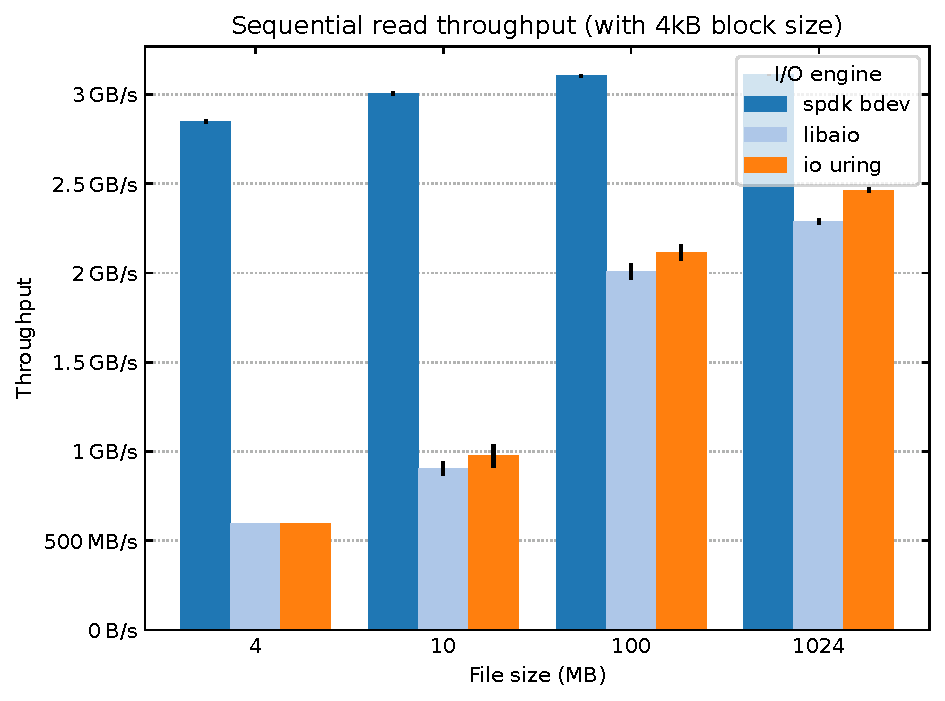
\includegraphics[width=\linewidth]{../measurements/npf/experiments/spdk/bs-4K/graphs/read-BANDWIDTH.pdf}
        \caption{Throughput of sequential read operations with 4kB block size}
        \label{fig:read-bandwidth-4K}
    \end{minipage}
    \hfill
    \begin{minipage}{0.495\columnwidth}
        \centering
        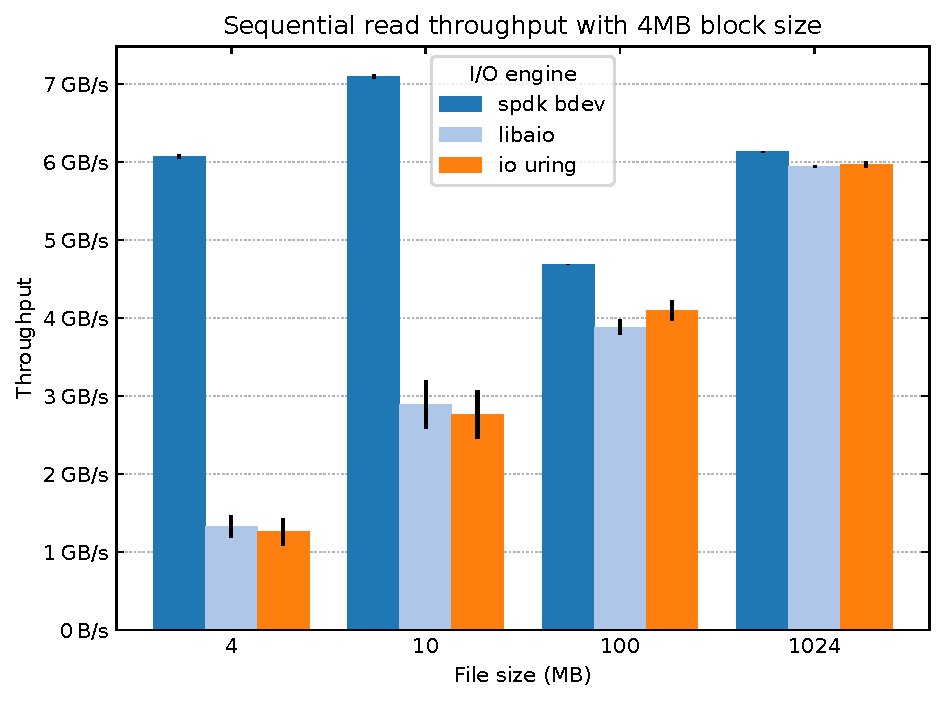
\includegraphics[width=\linewidth]{../measurements/npf/experiments/spdk/bs-4M/graphs/read-BANDWIDTH.pdf}
        \caption{Throughput of sequential read operations with 4MB block size}
        \label{fig:read-bandwidth-4M}
    \end{minipage}
\end{figure}

Looking at figure \ref{fig:read-bandwidth-4M} which illustrates throughput with 4 megabytes block size, we can observe that througput of all engines increase compared to 4kB block size. \acrshort{spdk} is consistent for all file size, with an average throughput of 6.73 GB/s (maximum achived is 6.75 GB/s). This throughput is close to the vendor theoretical speed of 7 GB/s. Kernel-path engines are still bottlenecked at small file size (4MB and 10MB), with an average throughput of respectively 1.53 GB/s and 2.01 GB/s, thus making \acrshort{spdk} 4.4 times faster than kernel-path engines. At larger file size (100MB and 1GB), kernel-path engines are able to achieve a mean throughput of 3.31 GB/s and 5.43 GB/s respectively, thus making \acrshort{spdk} 1.24 to 2.03 times faster than kernel-path engines. Standard deviation of \acrshort{spdk} is also significantly lower than kernel-path engines, ranging from 11.97 MB/s to 16.74 MB/s while kernel-path engines range from 96.58 MB/s to 218.24 MB/s. The results are summarized in table \ref{tab:stats-bandwidth-4M}.

We can conclude that \acrshort{spdk} is able to achieve higher throughput for sequential read operations with lower standard deviation than kernel-path engines, especially at small file size. It also follows the same order of magnitude for small file size regardless of block size, and is able to achieve close to vendor theoretical speed with large block size.


\subsubsection{Sequential write}

For sequential write with block size of 4 kB (figure \ref{fig:write-bandwidth-4K}), we can observe that \acrshort{spdk} is more stable in its mean output, reaching 6.25 GB/s with standard deviation of 35.09 MB/s to 59.09 MB/s. Kernel-path engines are capped at 2.1 GB/s in their best case, with standard deviation of 35.37 MB/s to 353.55 MB/s. Unlike read operations, write operations are bounded by the device NAND program time rather than \acrshort{pcie} bandwidth, so these numbers must also account eventual SLC caching. The results are summarized in table \ref{tab:stats-write-bandwidth-4K}.

\begin{figure}[htbp]
    \centering
    \begin{minipage}{0.495\columnwidth}
        \centering
        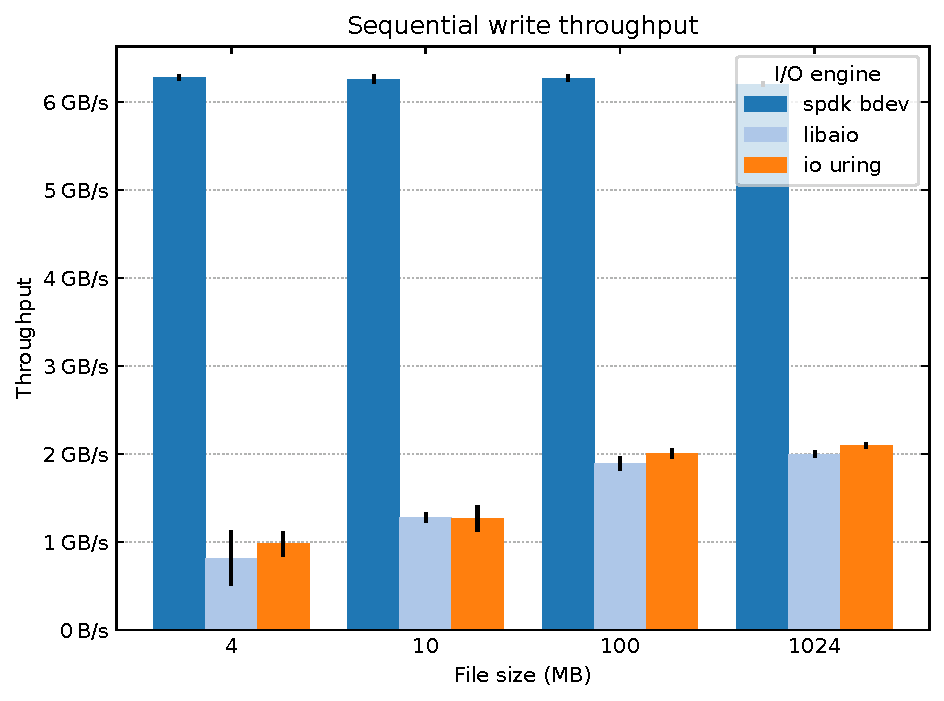
\includegraphics[width=\linewidth]{../measurements/npf/experiments/spdk/bs-4K/graphs/write-BANDWIDTH.pdf}
        \caption{Throughput of sequential write operations with 4kB block size}
        \label{fig:write-bandwidth-4K}
    \end{minipage}
    \hfill
    \begin{minipage}{0.495\columnwidth}
        \centering
        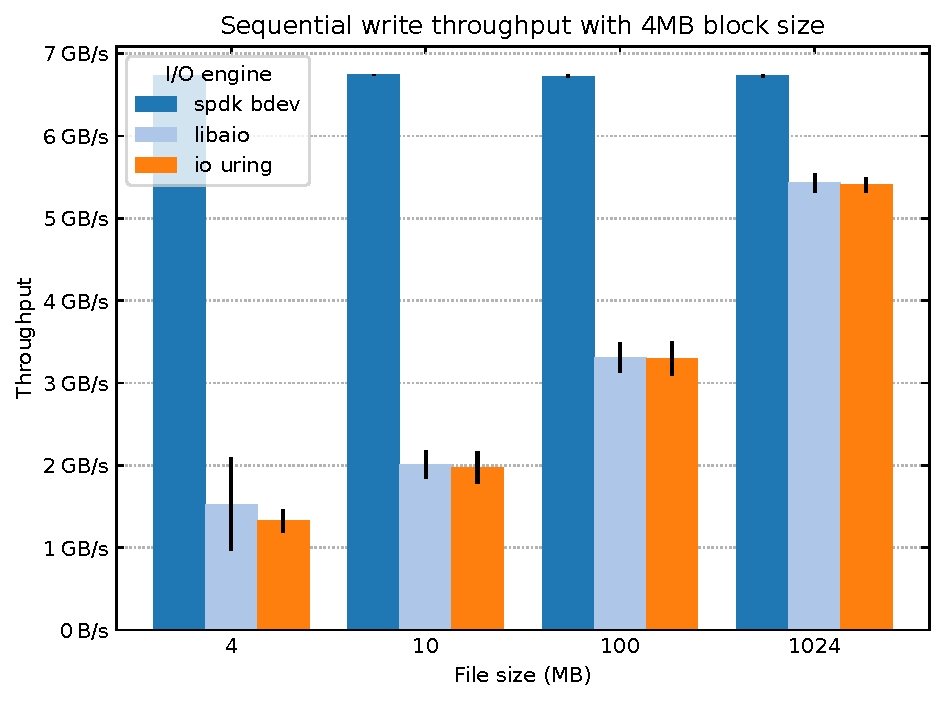
\includegraphics[width=\linewidth]{../measurements/npf/experiments/spdk/bs-4M/graphs/write-BANDWIDTH.pdf}
        \caption{Throughput of sequential write operations with 4MB block size}
        \label{fig:write-bandwidth-4M}
    \end{minipage}
\end{figure}

Figure \ref{fig:write-bandwidth-4M} shows the throughput of sequential write operations with 4MB block size. At this block size, \acrshort{spdk} has an higher average throughput of 6.73 GB/s with standard deviation of 11.97 MB/s to 16.74 MB/s, while kernel-path engines are capped at 5.43 GB/s with standard deviation of 96.58 MB/s to 595.86 MB/s.

While some configurations are able to exceed the vendor theoretical speed of 6.5 GB/s, caution should be taken as even if not specified by the vendor, the disk can use a dynamic \acrshort{pslc} write cache to achieve higher throughput. This is why we ran a time-based test of 300 seconds and ramp time of 30 seconds to evict eventual SLC caching in subsection \ref{subsec:slc-caching}.

\subsubsection{Random read and write}

    TO-DO

\subsection{Cost per I/O operation}

    Previous results show that kernel-path engines are impacted by the block size. We can compute the \acrfull{iops}  by dividing the throughput by the block size. Below is a table summarizing the average \acrshort{iops} for previous tests. The results show that \acrshort{spdk} is able to achieve higher \acrshort{iops} than kernel-path engines, especially at small block size. This is due to the fact that \acrshort{spdk} bypasses the kernel and directly accesses the device, while kernel-path engines have to go through the kernel, which adds overhead.

    \begin{table}[htbp]
        \centering
        \caption{Average \acrshort{iops} for all operations with 4kB and 4MB block size}
        \label{tab:stats-iops}
            \begin{tabularx}{\columnwidth}{@{}l l X X X@{}}
            \toprule
            \textbf{Block size} & \textbf{Operations} & \texttt{io\_uring} & \texttt{libaio} & \texttt{spdk\_bdev}\\
            \midrule
            \textbf{4kB} & Sequential Read & 397.03 kIOPS & 374.2 kIOPS & 1.56 MIOPS \\
            \textbf{4kB} & Random Read & 382.62 kIOPS & 355.03 kIOPS & 742.92 kIOPS \\
            \textbf{4kB} & Sequential Write & 397.03 kIOPS & 374.2 kIOPS & 1.56 MIOPS \\
            \textbf{4kB} & Random Write & 361.5 kIOPS & 339.55 kIOPS & 590.92 kIOPS \\
            \midrule
            \textbf{4MB} & Sequential Read & 384.53 IOPS & 362.57 IOPS & 753.92 kIOPS \\
            \textbf{4MB} & Random Read & 822.49 IOPS & 834.12 IOPS & 1.46 kIOPS \\
            \textbf{4MB} & Sequential Write & 750.63 IOPS & 767.51 IOPS & 1.68 kIOPS \\
            \textbf{4MB} & Random Write & 750.63 IOPS & 767.51 IOPS & 1.68 kIOPS \\
            \bottomrule
            \end{tabularx}
    \end{table}

    % \begin{figure}[htbp]
    %     \centering
    %     \begin{minipage}{0.495\columnwidth}
    %         \centering
    %         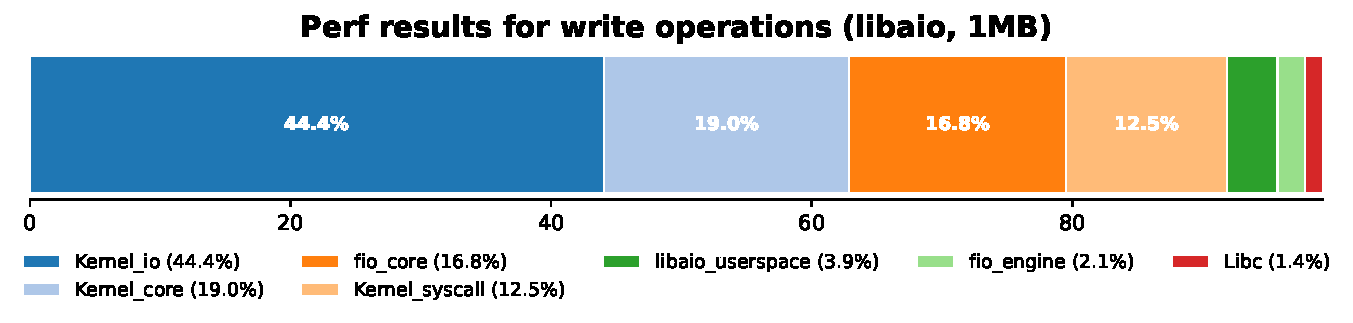
\includegraphics[width=\linewidth]{../measurements/perf/pdf/perf_libaio_write_20261028_154323.pdf}
    %         \caption{Perf of sequential write operations with 4kB block size and 1MB file size}
    %         \label{fig:perf-write-4k-1M}
    %     \end{minipage}
    %     \hfill
    %     \begin{minipage}{0.495\columnwidth}
    %         \centering
    %         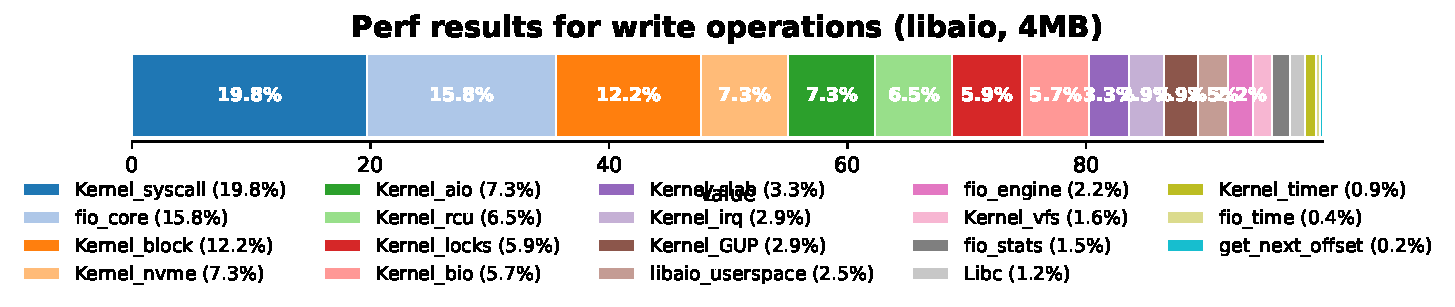
\includegraphics[width=\linewidth]{../measurements/perf/pdf/perf_libaio_4_write_20261028_171603.pdf}
    %         \caption{Throughput of sequential write operations with 4kB block size and 4MB file size}
    %         \label{fig:perf-write-4k-4M}
    %     \end{minipage}
    % \end{figure}
    \begin{figure}[htbp]
        \centering
        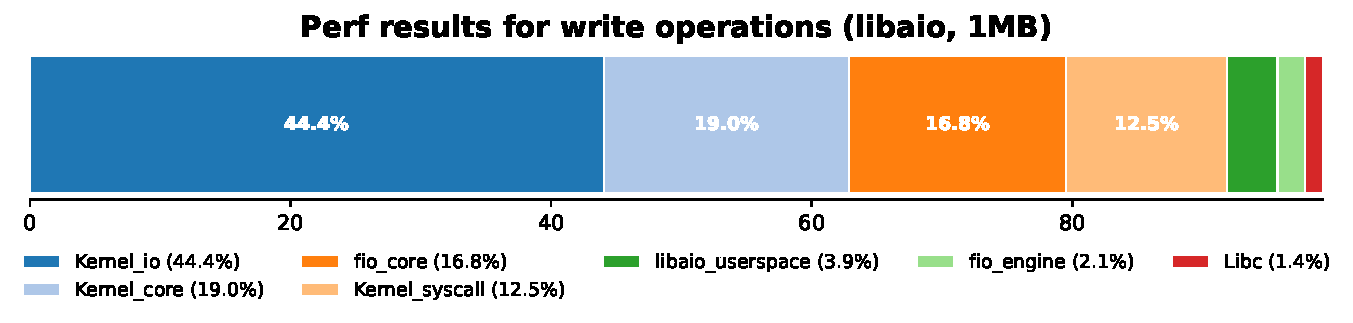
\includegraphics[width=\columnwidth]{../measurements/perf/pdf/perf_libaio_write_20261028_154323.pdf}
        \caption{Perf of sequential write operations with 4kB block size and 1MB file size with \texttt{libaio}}
        \label{fig:perf-write-libaio-4k-1M}
    \end{figure}

    \begin{figure}[htbp]
        \centering
        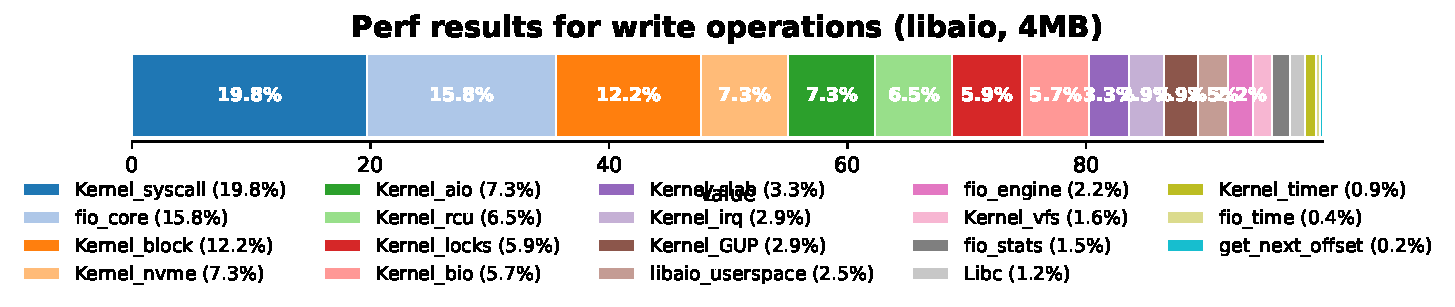
\includegraphics[width=\columnwidth]{../measurements/perf/pdf/perf_libaio_4_write_20261028_171603.pdf}
        \caption{Perf of sequential write operations with 4kB block size and 4MB file size with \texttt{libaio}}
        \label{fig:perf-write-libaio-4k-4M}
    \end{figure}

    \begin{figure}[htbp]
        \centering
        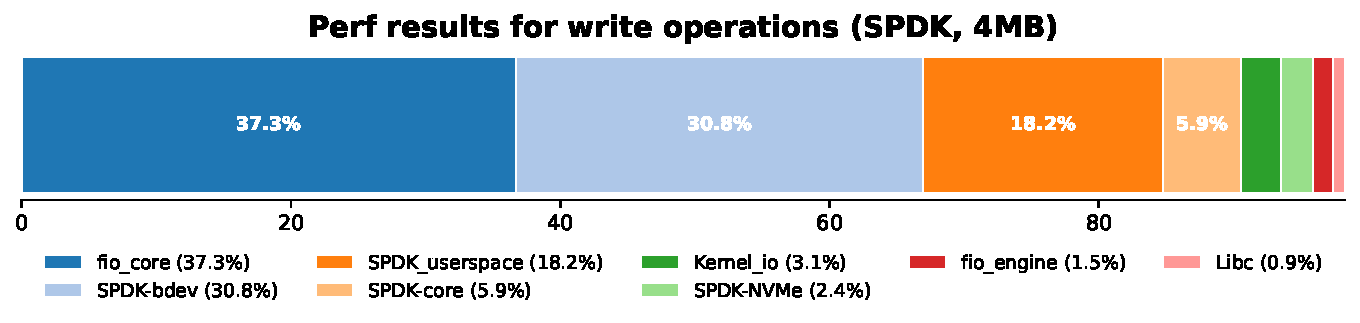
\includegraphics[width=\columnwidth]{../measurements/perf/bs-4K/pdf/perf_spdk_bdev_4_write_20261104_182456.pdf}
        \caption{Perf of sequential write operations with 4kB block size and 4MB file size with SPDK}
        \label{fig:perf-write-spdk-4k-4M}
    \end{figure}

    
    For example, for sequential read operations with 4kB block size, \acrshort{spdk} achieves on average 753.92 k\acrshort{iops} while kernel-path engines achieve on average 362.57 k\acrshort{iops} for \texttt{libaio} and 384.53 k\acrshort{iops} for \texttt{io\_uring}, nearly 2 times less. For 4MB block size, \acrshort{spdk} got on average 1.5 K\acrshort{iops} while \texttt{io\_uring} got 880.83 \acrshort{iops} and \texttt{libaio} got 878.34 \acrshort{iops}, nearly 1.7 times less.
    
    Figures \ref{fig:perf-write-4k-1M} and \ref{fig:perf-write-4k-4M} show the \texttt{perf} of sequential write operations with 4kB block size and 1MB or 4MB file size respectively. Up to 20 \% of the CPU time is spent on system calls. Detailed classification of the CPU time is available in table \ref{tab:perf-categories}.

\subsection{SLC cache} \label{subsec:slc-caching}

    TO-DO

    \begin{figure}[htbp]
        \centering
        \begin{minipage}{0.495\columnwidth}
            \centering
            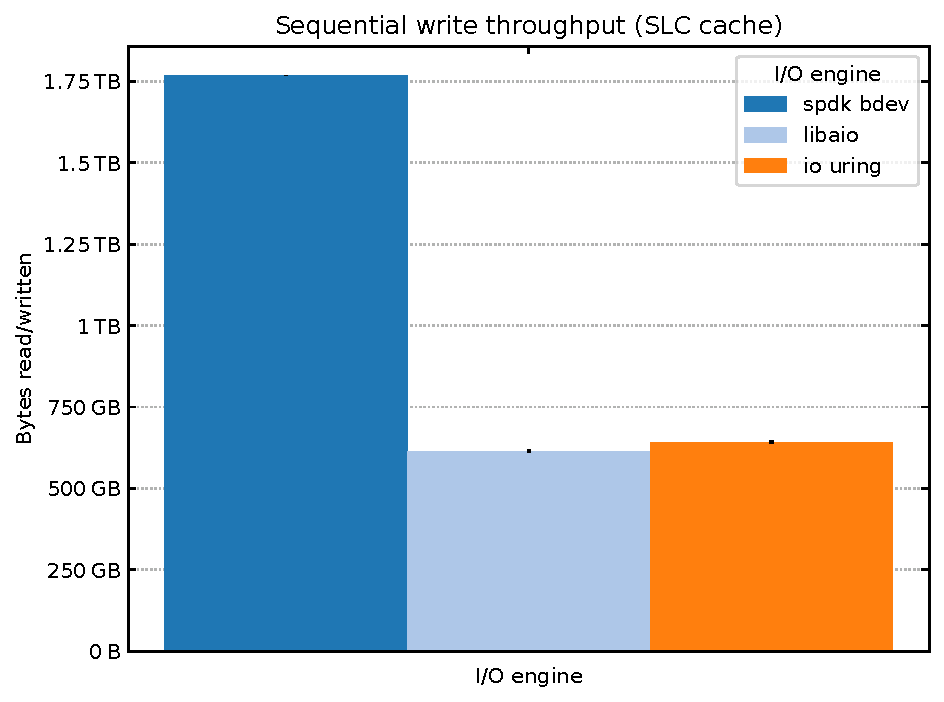
\includegraphics[width=\linewidth]{../measurements/npf/experiments/spdk/slc/graphs/write-IO_BYTES.pdf}
            \caption{Throughput of sequential write operations with 4kB block size and 1MB file size}
            \label{fig:slc-write-iobytes}
        \end{minipage}
        \hfill
        \begin{minipage}{0.495\columnwidth}
            \centering
            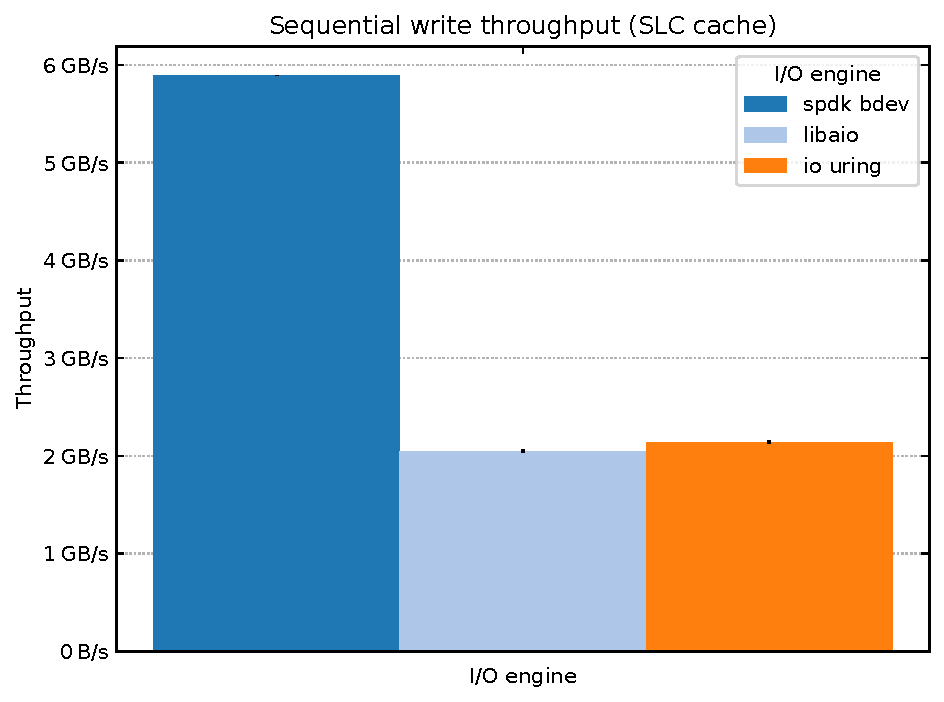
\includegraphics[width=\linewidth]{../measurements/npf/experiments/spdk/slc/graphs/write-BANDWIDTH.pdf}
            \caption{Throughput of sequential write operations with 4kB block size and 4MB file size}
            \label{fig:slc-write-bandwidth}
        \end{minipage}
    \end{figure}

\subsection{Latency} \label{subsec:disk-latency}

    TO-DO


\nt{Expland the discussion}
\subsection{Multiple cores} \label{subsec:disk-multicore}

    TO-DO
    
\section{NVMe-over-Fabrics performances}

    In this section we evaluate the throughput and latency of NVMe-over-Fabrics with Linux kernel on disk A. The tests evaluate both \acrshort{tcp} and \acrshort{rdma} transport. The tests are made with \texttt{\acrshort{fio}} \cite{noauthor_kernelgitaxboefiogit_nodate} with \texttt{io\_uring} engine. Queue depth is fixed to 64.

    \subsection{Throughput}

        \begin{figure}[htbp]
        \centering
        \begin{minipage}{0.495\columnwidth}
            \centering
            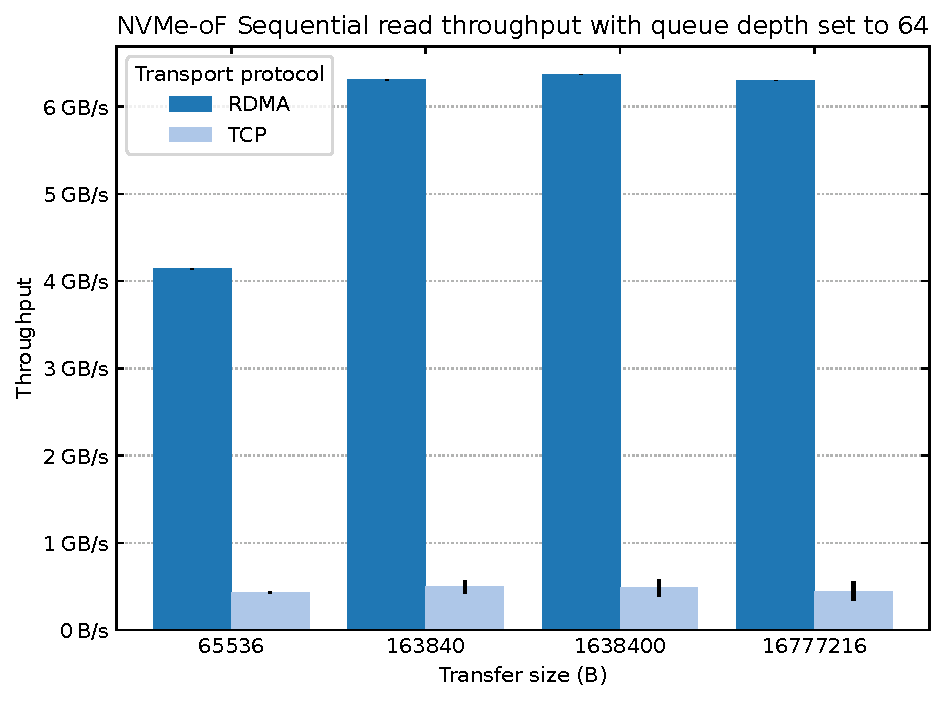
\includegraphics[width=\linewidth]{../measurements/npf/experiments/spdk/nvme-of/graphs/-read-BANDWIDTH.pdf}
            \caption{Throughput of sequential read operations for NVMe-over-Fabrics with large file size}
            \label{fig:nmve-of-read-bandwidth}
        \end{minipage}
        \hfill
        \begin{minipage}{0.495\columnwidth}
            \centering
            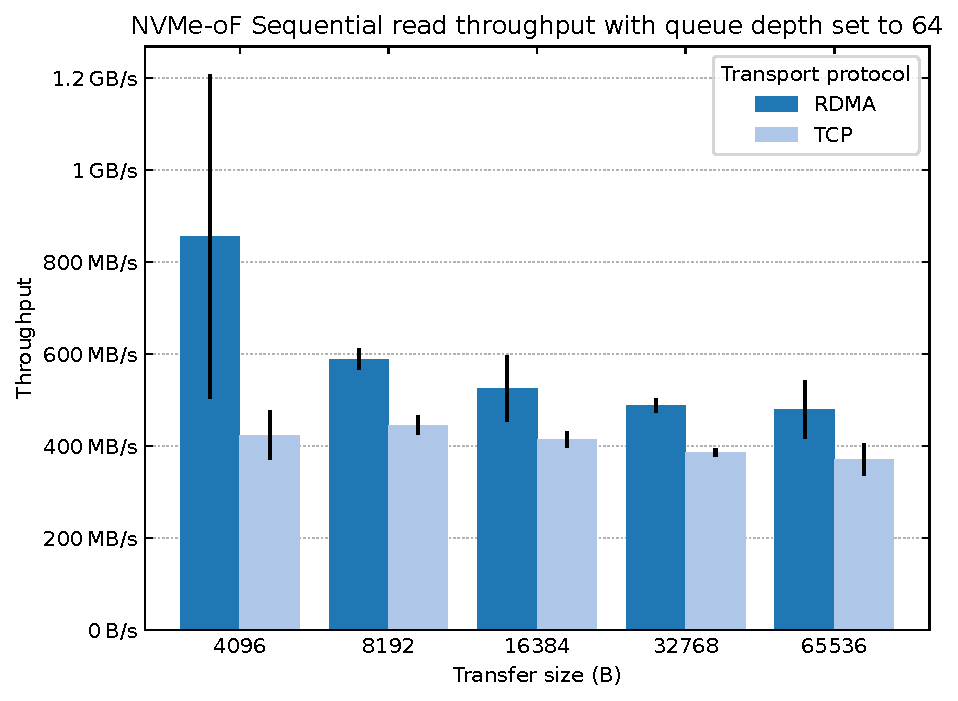
\includegraphics[width=\linewidth]{../measurements/npf/experiments/spdk/nvme-of/graphs/small-read-BANDWIDTH.pdf}
            \caption{Throughput of sequential read operations for NVMe-over-Fabrics with small file size}
            \label{fig:nmve-of-read-bandwidth-small}
        \end{minipage}
    \end{figure}

\section{lighttpd performances}

We benchmarked the \acrshort{http} server \texttt{lighttpd} original version (1.4.32) \cite{lighttpd_1.4.32_news,lighttpd_1.4.32_github} in order to analyze the difference between the original version and the IO-TCP version. The benchmark is made with \texttt{wrk} \cite{glozer_wgwrk_2026}. To be fair with IO-TCP, we restrict the \texttt{lighttpd} to a single core. Figures \ref{fig:lighttpd-x86} and \ref{fig:lighttpd-arm} show the throughput of \texttt{lighttpd} on Frodo server (x86\_64 core) and on SmartNIC (ARM Cortex-A72 core) respectively. We observe that a single core on Frodo is nearly able to saturate the disk bandwidth.

\begin{figure}[htbp]
    \centering
    \begin{minipage}{0.495\columnwidth}
        \centering
        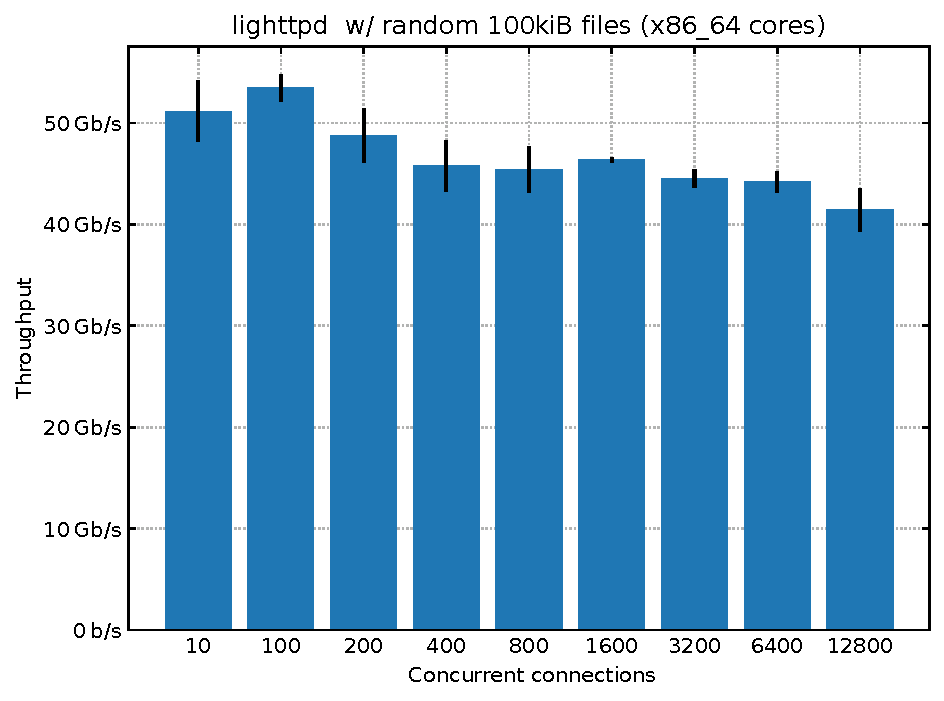
\includegraphics[width=\linewidth]{../measurements/npf/experiments/lighttpd/frodo-random-100k-BANDWIDTH.pdf}
        \caption{Throughput of lighttpd on Frodo server (x86\_64 core)}
        \label{fig:lighttpd-x86}
    \end{minipage}
    \hfill
    \begin{minipage}{0.495\columnwidth}
        \centering
        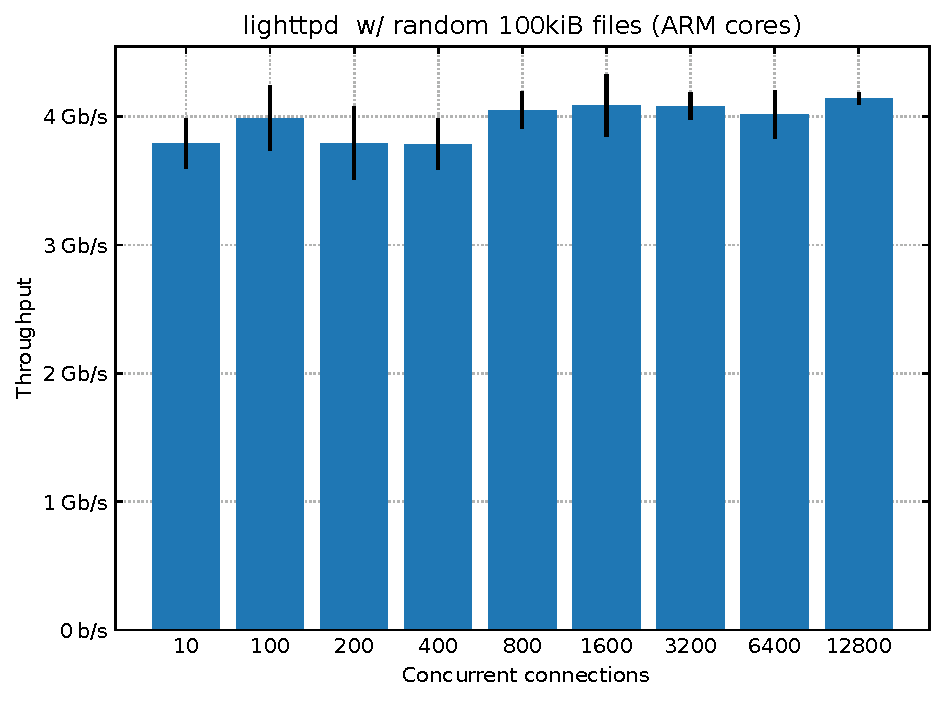
\includegraphics[width=\linewidth]{../measurements/npf/experiments/lighttpd/bluefield-random-100k-BANDWIDTH.pdf}
        \caption{Throughput of lighttpd on SmartNIC (ARM Cortex-A72 core)}
        \label{fig:lighttpd-arm}
    \end{minipage}
\end{figure}


\section{IO-TCP performances}


\section{Implementation performances}
 


\chapter{Conclusion and future work} \label{ch:conclusion}

    TODO

\chapter*{Appendix : additional plots data} \label{ch:appendix-plots-data}
\pagenumbering{roman}
\setcounter{page}{1}

    \section{Disk performances}

\subsection{Read operations}

\begin{table}[H]
\centering
\caption{Statistical summary of figure \ref{fig:read-bandwidth-4K} : read throughput with 4kB block size}
\label{tab:stats-bandwidth-4K}
% \renewcommand{\arraystretch}{1.0}
\resizebox{\columnwidth}{!}{%
\begin{tabular}{@{}l l c c c c c@{}}
\toprule
\textbf{Engine} & \textbf{Size (MB)} & \textbf{Mean} & \textbf{Std. Dev.} & \textbf{Min} & \textbf{Median} & \textbf{Max} \\
\midrule
\midrule
\textbf{io\_uring} & 4 & 584.21MB/s & 33.50MB/s & 524.29MB/s & 599.19MB/s & 599.19MB/s \\
\textbf{io\_uring} & 10 & 956.43MB/s & 61.94MB/s & 873.81MB/s & 953.25MB/s & 1.05GB/s \\
\textbf{io\_uring} & 100 & 2.01GB/s & 41.52MB/s & 1.94GB/s & 2.02GB/s & 2.06GB/s \\
\textbf{io\_uring} & 1024 & 2.38GB/s & 55.04MB/s & 2.30GB/s & 2.36GB/s & 2.45GB/s \\
\midrule
\textbf{libaio} & 4 & 584.21MB/s & 33.50MB/s & 524.29MB/s & 599.19MB/s & 599.19MB/s \\
\textbf{libaio} & 10 & 905.59MB/s & 43.51MB/s & 873.81MB/s & 873.81MB/s & 953.25MB/s \\
\textbf{libaio} & 100 & 1.89GB/s & 45.43MB/s & 1.84GB/s & 1.91GB/s & 1.94GB/s \\
\textbf{libaio} & 1024 & 2.25GB/s & 13.68MB/s & 2.24GB/s & 2.25GB/s & 2.27GB/s \\
\midrule
\textbf{spdk\_bdev} & 4 & 2.63GB/s & 10.07MB/s & 2.62GB/s & 2.62GB/s & 2.64GB/s \\
\textbf{spdk\_bdev} & 10 & 2.98GB/s & 313.99kB/s & 2.98GB/s & 2.98GB/s & 2.98GB/s \\
\textbf{spdk\_bdev} & 100 & 2.51GB/s & 1.49MB/s & 2.51GB/s & 2.51GB/s & 2.51GB/s \\
\textbf{spdk\_bdev} & 1024 & 3.00GB/s & 12.46MB/s & 2.99GB/s & 3.01GB/s & 3.01GB/s \\
\bottomrule
\end{tabular}%
}
\end{table}

\begin{table}[H]
\centering
\caption{Statistical summary of figure \ref{fig:read-bandwidth-4M} : read throughput with 4MB block size}
\label{tab:stats-bandwidth-4M}
% \renewcommand{\arraystretch}{1.0}
\resizebox{\columnwidth}{!}{%
\begin{tabular}{@{}l l c c c c c@{}}
\toprule
\textbf{Engine} & \textbf{Size (MB)} & \textbf{Mean} & \textbf{Std. Dev.} & \textbf{Min} & \textbf{Median} & \textbf{Max} \\
\midrule
\midrule
\textbf{io\_uring} & 4 & 1.33GB/s & 147.37MB/s & 1.05GB/s & 1.40GB/s & 1.40GB/s \\
\textbf{io\_uring} & 10 & 1.97GB/s & 202.60MB/s & 1.68GB/s & 2.10GB/s & 2.10GB/s \\
\textbf{io\_uring} & 100 & 3.30GB/s & 218.24MB/s & 2.69GB/s & 3.38GB/s & 3.38GB/s \\
\textbf{io\_uring} & 1024 & 5.41GB/s & 96.58MB/s & 5.32GB/s & 5.36GB/s & 5.56GB/s \\
\midrule
\textbf{libaio} & 4 & 1.53GB/s & 595.86MB/s & 262.14MB/s & 1.40GB/s & 2.10GB/s \\
\textbf{libaio} & 10 & 2.01GB/s & 176.85MB/s & 1.68GB/s & 2.10GB/s & 2.10GB/s \\
\textbf{libaio} & 100 & 3.31GB/s & 196.16MB/s & 2.76GB/s & 3.38GB/s & 3.38GB/s \\
\textbf{libaio} & 1024 & 5.43GB/s & 122.58MB/s & 5.24GB/s & 5.38GB/s & 5.62GB/s \\
\midrule
\textbf{spdk\_bdev} & 4 & 6.73GB/s & 11.97MB/s & 6.72GB/s & 6.73GB/s & 6.75GB/s \\
\textbf{spdk\_bdev} & 10 & 6.74GB/s & 12.38MB/s & 6.72GB/s & 6.74GB/s & 6.75GB/s \\
\textbf{spdk\_bdev} & 100 & 6.72GB/s & 16.74MB/s & 6.70GB/s & 6.72GB/s & 6.75GB/s \\
\textbf{spdk\_bdev} & 1024 & 6.73GB/s & 14.98MB/s & 6.71GB/s & 6.73GB/s & 6.75GB/s \\
\bottomrule
\end{tabular}%
}
\end{table}

\subsection{Write operations}


\begin{table}[H]
\centering
\caption{Statistical summary of figure \ref{fig:write-bandwidth-4K} : write throughput with 4kB block size}
\label{tab:stats-write-bandwidth-4K}
% \renewcommand{\arraystretch}{1.0}
\resizebox{\columnwidth}{!}{%
\begin{tabular}{@{}l l c c c c c@{}}
\toprule
\textbf{Engine} & \textbf{Size (MB)} & \textbf{Mean} & \textbf{Std. Dev.} & \textbf{Min} & \textbf{Median} & \textbf{Max} \\
\midrule
\midrule
\textbf{io\_uring} & 4 & 1.05GB/s & 0.00B/s & 1.05GB/s & 1.05GB/s & 1.05GB/s \\
\textbf{io\_uring} & 10 & 1.39GB/s & 102.56MB/s & 1.31GB/s & 1.31GB/s & 1.50GB/s \\
\textbf{io\_uring} & 100 & 1.71GB/s & 165.90MB/s & 1.57GB/s & 1.61GB/s & 1.91GB/s \\
\textbf{io\_uring} & 1024 & 2.10GB/s & 55.96MB/s & 2.03GB/s & 2.08GB/s & 2.16GB/s \\
\midrule
\textbf{libaio} & 4 & 608.59MB/s & 202.29MB/s & 246.72MB/s & 699.05MB/s & 699.05MB/s \\
\textbf{libaio} & 10 & 991.38MB/s & 52.21MB/s & 953.25MB/s & 953.25MB/s & 1.05GB/s \\
\textbf{libaio} & 100 & 1.87GB/s & 87.03MB/s & 1.78GB/s & 1.84GB/s & 1.98GB/s \\
\textbf{libaio} & 1024 & 2.02GB/s & 35.20MB/s & 1.98GB/s & 2.01GB/s & 2.07GB/s \\
\midrule
\textbf{spdk\_bdev} & 4 & 5.16GB/s & 2.48GB/s & 731.38MB/s & 6.24GB/s & 6.34GB/s \\
\textbf{spdk\_bdev} & 10 & 6.28GB/s & 62.16MB/s & 6.23GB/s & 6.24GB/s & 6.36GB/s \\
\textbf{spdk\_bdev} & 100 & 6.27GB/s & 49.40MB/s & 6.23GB/s & 6.25GB/s & 6.33GB/s \\
\textbf{spdk\_bdev} & 1024 & 6.25GB/s & 35.50MB/s & 6.19GB/s & 6.26GB/s & 6.28GB/s \\
\bottomrule
\end{tabular}%
}
\end{table}

\begin{table}[H]
\centering
\caption{Statistical summary of figure \ref{fig:write-bandwidth-4M} : write throughput with 4MB block size}
\label{tab:stats-write-bandwidth-4M}
% \renewcommand{\arraystretch}{1.0}
\resizebox{\columnwidth}{!}{%
\begin{tabular}{@{}l l c c c c c@{}}
\toprule
\textbf{Engine} & \textbf{Size (MB)} & \textbf{Mean} & \textbf{Std. Dev.} & \textbf{Min} & \textbf{Median} & \textbf{Max} \\
\midrule
\midrule
\textbf{io\_uring} & 4 & 1.33GB/s & 147.37MB/s & 1.05GB/s & 1.40GB/s & 1.40GB/s \\
\textbf{io\_uring} & 10 & 1.97GB/s & 202.60MB/s & 1.68GB/s & 2.10GB/s & 2.10GB/s \\
\textbf{io\_uring} & 100 & 3.30GB/s & 218.24MB/s & 2.69GB/s & 3.38GB/s & 3.38GB/s \\
\textbf{io\_uring} & 1024 & 5.41GB/s & 96.58MB/s & 5.32GB/s & 5.36GB/s & 5.56GB/s \\
\midrule
\textbf{libaio} & 4 & 1.53GB/s & 595.86MB/s & 262.14MB/s & 1.40GB/s & 2.10GB/s \\
\textbf{libaio} & 10 & 2.01GB/s & 176.85MB/s & 1.68GB/s & 2.10GB/s & 2.10GB/s \\
\textbf{libaio} & 100 & 3.31GB/s & 196.16MB/s & 2.76GB/s & 3.38GB/s & 3.38GB/s \\
\textbf{libaio} & 1024 & 5.43GB/s & 122.58MB/s & 5.24GB/s & 5.38GB/s & 5.62GB/s \\
\midrule
\textbf{spdk\_bdev} & 4 & 6.73GB/s & 11.97MB/s & 6.72GB/s & 6.73GB/s & 6.75GB/s \\
\textbf{spdk\_bdev} & 10 & 6.74GB/s & 12.38MB/s & 6.72GB/s & 6.74GB/s & 6.75GB/s \\
\textbf{spdk\_bdev} & 100 & 6.72GB/s & 16.74MB/s & 6.70GB/s & 6.72GB/s & 6.75GB/s \\
\textbf{spdk\_bdev} & 1024 & 6.73GB/s & 14.98MB/s & 6.71GB/s & 6.73GB/s & 6.75GB/s \\
\bottomrule
\end{tabular}%
}
\end{table} 

\printbibliography[heading=bibintoc]

% Back cover page
\backcoverpage

\end{document}
